%%% File-Information {{{
%%% Filename: template_bericht.tex
%%% Purpose: lab report, technical report, project report
%%% Time-stamp: <2004-06-22 23:36:32 xx>
%%% Authors: The LaTeX@TUG-Team [http://latex.tugraz.at/]:
%%%          Karl Voit (vk), Michael Prokop (mp), Stefan Sollerer (ss)
%%% History:
%%%   20040625 (vk,ss) initial version
%%%
%%% Notes:
%%%
%%%
%%%
%%% }}}
%%%%%%%%%%%%%%%%%%%%%%%%%%%%%%%%%%%%%%%%%%%%%%%%%%%%%%%%%%%%%%%%%%%%%%%%%%%%%%%%
%%% main document {{{

\documentclass[
a4paper,     %% defines the paper size: a4paper (default), a5paper, letterpaper, ...
% landscape,   %% sets the orientation to landscape
% twoside,     %% changes to a two-page-layout (alternatively: oneside)
% twocolumn,   %% changes to a two-column-layout
 headsepline, %% add a horizontal line below the column title
% footsepline, %% add a horizontal line above the page footer
% titlepage,   %% only the titlepage (using titlepage-environment) appears on the first page (alternatively: notitlepage)
 halfparskip,     %% insert an empty line between two paragraphs (alternatively: halfparskip, ...)
% leqno,       %% equation numbers left (instead of right)
 fleqn,       %% equation left-justified (instead of centered)
% tablecaptionabove, %% captions of tables are above the tables (alternatively: tablecaptionbelow)
% draft,       %% produce only a draft version (mark lines that need manual edition and don't show graphics)
% 10pt         %% set default font size to 10 point
% 11pt         %% set default font size to 11 point
12pt         %% set default font size to 12 point
]{scrartcl}  %% article, see KOMA documentation (scrguide.dvi)

\usepackage[english,german]{babel} 
\usepackage[latin1]{inputenc}

\usepackage[T1]{fontenc}
\usepackage{ae,aecompl}

\usepackage{amsmath,amssymb,amstext}
\usepackage{units}
\usepackage{scrpage2}
\usepackage{graphicx}

%%% \mygraphics{}{}{}
%% usage:   \mygraphics{width}{filename_without_extension}{caption}
%% example: \mygraphics{0.7\textwidth}{rolling_grandma}{This is my grandmother on inlinescates}
%% requires: package graphicx
%% provides: including centered pictures/graphics with a boldfaced caption below
%% 
\newcommand{\mygraphics}[3]{
  \begin{center}
    \includegraphics[width=#1, keepaspectratio=true]{#2} \\
    \textbf{#3}
  \end{center}
}

\subject{CVME Seminar}   %% subject which appears above titlehead
\title{Outlier Detection}
\author{Dominik Sch�rkhuber}
\date{Vienna University of Technology, May 2015}

\begin{document}
 \pagenumbering{roman} %% small roman page numbers
 \maketitle
 \tableofcontents
 \listoffigures
 \listoftables
 \pagenumbering{arabic} %% normal page numbers (include it, if roman was used above)

\section{Introduction}
Outlier Detection is the identification of data which is not conform to an expected pattern. Unlike in clustering, where items of common behavior are grouped together, and outliers may be seen as unwanted noise, we are actively searching with outlier detection methods for anomalies rather than common patterns in data. Outlier detection is a heavily researched topic and has in its generality a wide range of applications. Some examples are fault detection in safety critical systems, supervision of banking systems, video surveillance or intrusion detection in cyber security. In all those cases we want to automatically distinguish usual behavior from abnormal behavior, which may indicate a system breakdown, fraud, etc. Outliers may also be of use in a more positive way. For example human resource management may use outlier detection techniques to find people capable of a very diverse set of skills. From those examples we can conclude that in many cases abnormal data may be of great interest instead of data following a common pattern. 
Until now the very generic term data was used, we now want to closer specify how input data for outlier detection algorithms may look like. A single data instance consists of multiple attributes, similar to descriptors in image analysis. Data attributes can be classified in different types of data like binary, categorial, discrete or continous data. Each data instance may contain one (univariate) or multiple (multivariate) attributes. In the multivariate case the attribute types may be coherent or different among attributes. 
Consider Fig.~\ref{fig:outlierExample} as an abstract example with input data in the attribute space $\mathbb{R}^2$. Each data point consists of two attributes $p=(x,y)$ with $x,y \in \mathbb{R}$. The data is split into several regions. $N_1$ and $N_2$ refer to normal regions, those points describe normal behavior. $O_1$ and $O_2$ are single outliers, $O_3$ is an outlying region. 

\begin{figure}
	\begin{center}
    	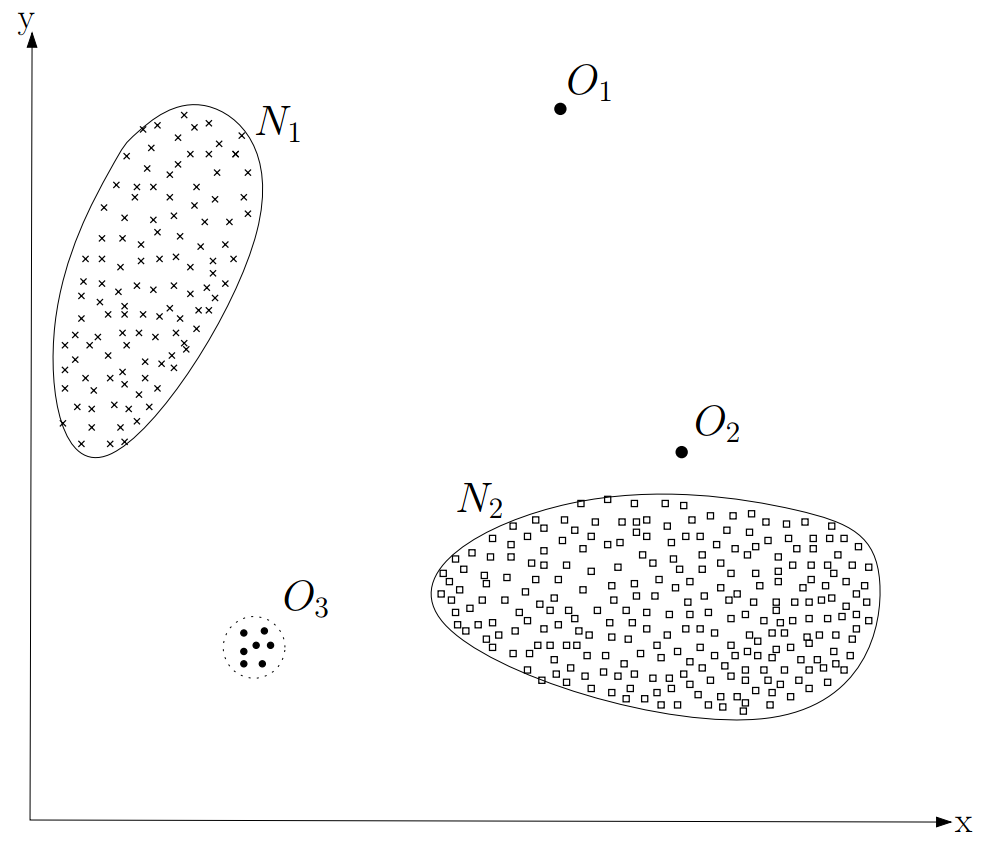
\includegraphics[width=0.5\textwidth]{images/outlier_example}
    \end{center}
	\caption{Example for Outlier Detection}
	\label{fig:outlierExample}
\end{figure}

\subsection{Types of supervision}
Outlier detection methods can be classified by their type of supervision. Besides the actual data instances an outlier detection algorithm may also use additional information for distinction of outliers from inliers. Such information can be class labels as they are used in pattern matching algorithms. The data instances of a training dataset is augumented with class information. This information enables us to generate a predictive model which may classify data instances of test data. Depending on how much a method utilizes this additional information we distinguish three classes of supervision. 
\\
\textit{Supervised methods} make heavy use of labeling information. These techniques require class (labeling) information for each normal and outlier point in the training dataset. Typically a predicitive model is built which enables the algorithm to classify further data points into normals or outliers. The main drawback of supervised methods is it may be very expensive to acquire correctly labeled training datasets. Depending on the field of use a human expert may be required to do a correct labeling or atleast correct a given automatic labeling of training data. 
\\
\textit{Semi-supervised methods} on the other hand only require labeling information for one class of points. Either only normal or abnormal behavior is captured by the training set. It is often very difficult to provide correct labels for both classes of points. For example in a network intrusion detection system it is usually impossible to model all possible attack vectors as outliers in a training dataset. Whereas information of normal use of the network may be automatically acquired. For this reason unsupervised methods with known sets of outliers are not very popular. Since normal behavior is easier to model techniques with known normal datasets are usually used. 
\\
\textit{Unsupervised methods} as a third method does not rely on any additional information. Therefore these methods are widely applicable since no additional information must be provided. Still we need some way of categorising input data points. For example statistic methods can be used to adapt a parametric distribution to normal and/or abnormal data. Based on a statistical test we may distinguish inliers from outliers. Also many techniques rely on the fact that normal data instances are occuring more frequently than abnormal data instances. Therefore frequently occuring patterns are classified as normal, whereas rare patterns are assumed to be abnormal. 

global vs local
labeling vs scoring = hard / soft
TypeI TypeII outliers

side products of clustering
categories of outlier detection methods

proximity based
angle based

\section{Outlier Detection in High Dimensional Data}


\section{Application of Outlier Detection Techniques}



\section{Identifying Density-based Local Outliers}


 \appendix  %% include it, if something (bibliography, index, ...) follows below
 \bibliographystyle{plain}

 \bibliography{projekt}

\end{document}

